\chapter{検出器量産と品質試験}

\section{組み立て工程}
現在モジュールの組み立て工程として以下が設定されている。
\begin{enumerate}
  \item プリント基板・ベアモジュール貼り付け
  \begin{itemize}
    \item hoge
  \end{itemize}
  \item ワイヤー配線
  \begin{itemize}
    \item hoge
  \end{itemize}
  \item ワイヤー保護
  \begin{itemize}
    \item hoge
  \end{itemize}
  \item パリレンコーティング
  \begin{itemize}
    \item hoge
  \end{itemize}
  \item 温度サイクル試験
  \begin{itemize}
    \item hoge
  \end{itemize}
  \item 低温耐久試験
  \begin{itemize}
    \item hoge
  \end{itemize}
\end{enumerate}

流れと各組み立て工程のイメージを図\ref{assembly_flow}に示す。
\begin{figure}[bpt]\centering
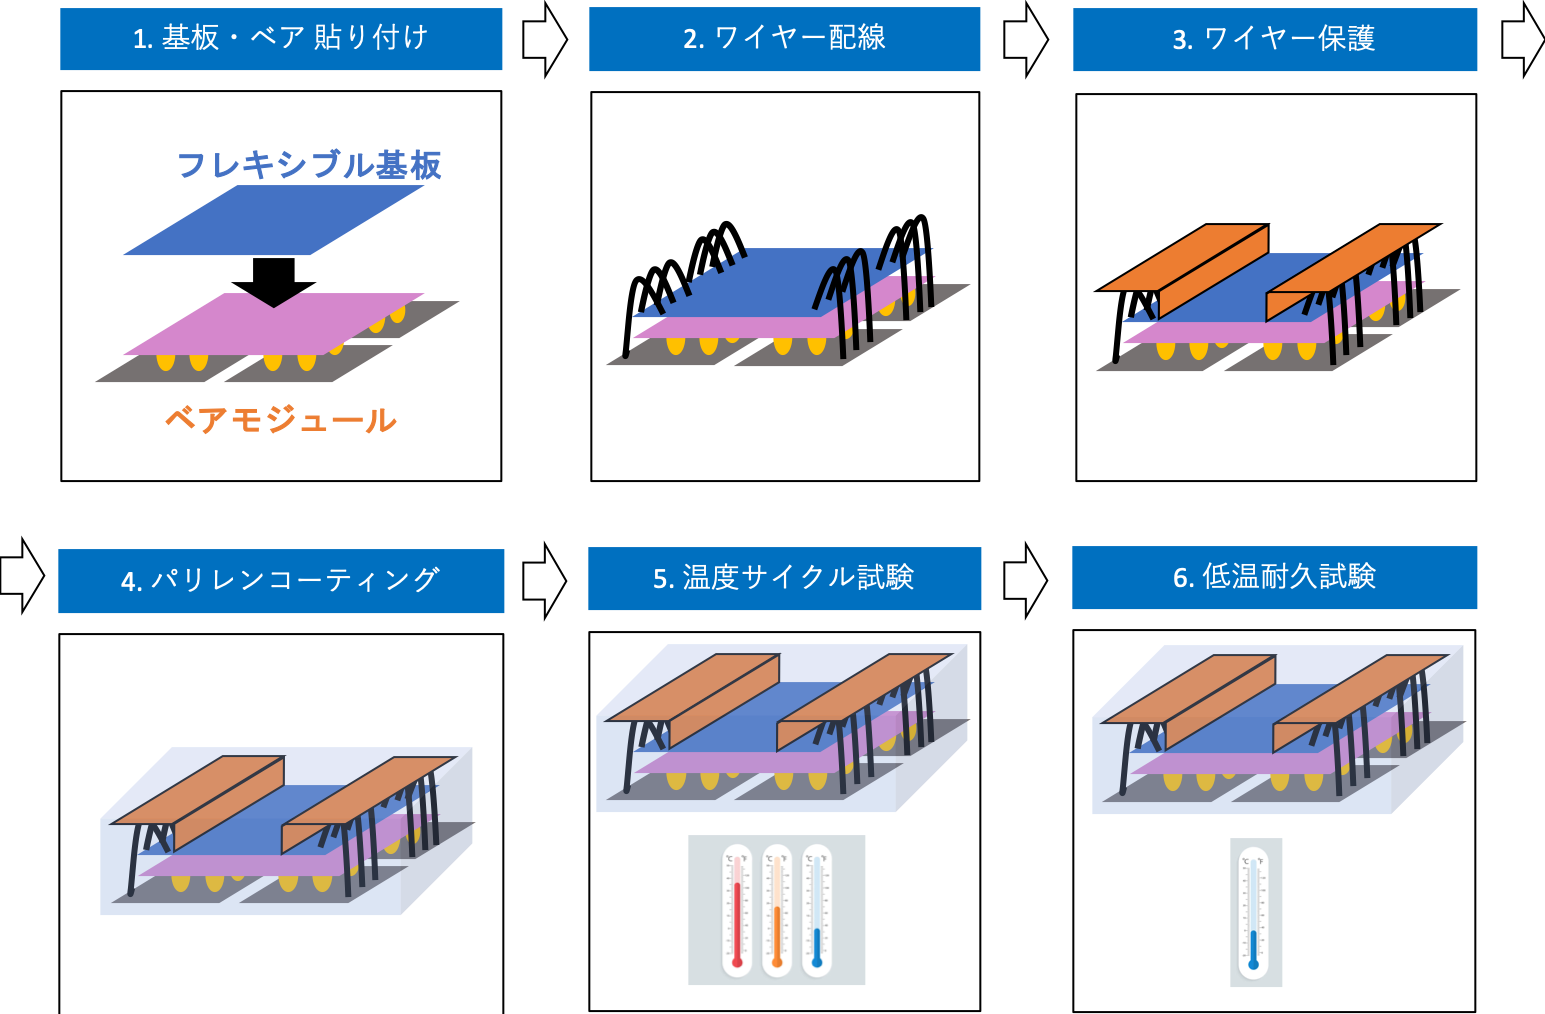
\includegraphics[width=14cm]{assembly_flow}
\caption[組み立て工程]{組み立て工程}
\label{assembly_flow}
\end{figure}

\section{品質試験}
各組み立て工程に対して、いくつかの品質試験を行う。行う品質試験の代表的なものを以下に示す。

\subsection{外観検査(Visual Inspection)}

\subsection{質量測定(Mass Measurement)}

\subsection{平坦性測定(Metrology)}

\subsection{センサー電流$-$電圧特性確認(Sensor IV)}

\subsection{FEチップ電流$-$電圧特性確認(SLDO VI)}

\subsection{読み出し試験}

\subsubsection{用いるSWとSetup}

\subsubsection{レジスタ書き換え(Chip Configuration)}

\subsubsection{試験項目詳細}
\begin{itemize}
  \item レジスタ読み出し(Register test)
  \item デジタル回路読み出し(Digital scan)
  \item アナログ回路読み出し(Analog scan)
  \item Threshold測定(Threshold scan)
  \item Thresholdグローバルレジスタ調整(Global threshold tuning)
  \item Thresholdピクセルレジスタ調整、再調整、精密調整(Pixel threshold tuning)
  \item ToTグローバルレジスタ調整(ToT tuning)
  \item ノイズ占有率測定(Noise scan)
  \item スタックピクセル測定(Stuck pixel scan)
  \item クロストーク測定(Crosstalk scan)
  \item バンプ接続確認測定(Disconnected bump scan)
  \item 外部トリガーを用いた測定(External trriger)
\end{itemize}
ここから1つ1つの詳細について説明する。
  
\subsubsection{Threshold調整とピクセル解析}
以下の流れで読み出しを行う。
\begin{itemize}
  \item デジタル回路読み出し
  \item アナログ回路読み出し
  \item Threshold測定
  \item Thresholdグローバルレジスタ調整
  \item Thresholdピクセルレジスタ調整
  \item ToTグローバルレジスタ調整
  \item Thresholdグローバルレジスタ再調整、精密調整
  \item Threshold測定
  \item スタックピクセル測定
  \item クロストーク測定
\end{itemize}

digital scan
・Explanation
・Output files


モジュール上のピクセルを解析し、各ピクセルが正常かどうかを判断する。
以下の評価基準で解析をし、不良ピクセルには評価基準に応じた評価名が付けられる

\begin{table}[tbp]
\begin{center}
\caption[ピクセル解析の評価基準]{ピクセル解析の評価基準\cite{3-1}}
\label{pixel_analysis_criteria}
  \begin{tabular}{|lll|} \hline
    評価名 & 読み出し項目 & 不良評価基準 \\ \hline
    Digital Dead      & Digital scan           & Occupancy < 1 \\ \hline
    Digital Bad       & Digital scan           & Occupancy < 98 or Occupancy > 102\\\hline 
    Merged Bump       & Analog scan            & Occupancy < 98 or Occupancy > 102 \\ 
                      & Crosstalk scan         & High Crosstalk\\ \hline
    Analog Dead       & Analog scan            & Occupancy < 1 \\ \hline
    Analog Bad        & Analog scan            & Occupancy < 98 or Occupancy > 102 \\ \hline
    Tuning Failed     & Threshold scan         & カイ二乗=0 \\ \hline
    Tuning Bad        & Threshold scan         & $\pm5\sigma$\\ 
                      & ToT scan               & 0 or 15 \\ \hline
    High ENC          & Threshold scan         & $\pm3\sigma$ \\ \hline
    Noisy             & Noise scan             & Occupancy > $10^{-6}$\\ \hline
    Disconnected Bump & Disconnected bump scan & 未決定 \\ 
                      & Source scan            & Occupancyが平均値の1$\%$ \\ \hline
    High Crosstalk    & Crosstalk scan         & Occupancy>0 with 25e(sync)\\
                      &                        & Occupancy>0 with 40e(lin and diff)\\ \hline 
  \end{tabular}
\end{center}
\end{table}

\subsubsection{簡易読み出し試験}
簡易読み出し試験では以下の項目を扱う。
\begin{itemize}
  \item レジスタ読み出し
  \item デジタル回路読み出し
  \item アナログ回路読み出し
  \item Threshold読み出し
  \item ToT読み出し
  \item バンプ接続確認読み出し
\end{itemize}

\subsubsection{バンプ接合確認試験(Bump bond quality)}
放射線源を用いてバンプ接合の確認を行う。

\subsection{各組み立て工程における品質試験}

各組み立て工程と品質試験項目を図\ref{stage_test_flow}に示す。
\begin{figure}[bpt]\centering

\includegraphics[width=10cm]{figure}
\caption[組み立て工程と対応する品質試験]{組み立て工程と対応する品質試験}
\label{stage_test_flow}
\end{figure}

\section{検出器量産と品質試験データ管理に対する要求}

読み出し試験については特にデータ管理が大変。
